%%%%%%%%%%%%%%%%%%%%%%%%%%%%%%%%%%%%%%%%%%%%%%%%%%%%%%%%%%%%%%%%%%%%%%%%%%%%%%%
% Chapter 'Adsorption - Water - silica gel pellet '
%%%%%%%%%%%%%%%%%%%%%%%%%%%%%%%%%%%%%%%%%%%%%%%%%%%%%%%%%%%%%%%%%%%%%%%%%%%%%%%
\subsection{Silica gel pellet }
%
%%%%%%%%%%%%%%%%%%%%%%%%%%%%%%%%%%%%%%%%%%%%%%%%%%%%%%%%%%%%%%%%%%%%%%%%%%%%%%%
%%%%%%%%%%%%%%%%%%%%%%%%%%%%%%%%%%%%%%%%%%%%%%%%%%%%%%%%%%%%%%%%%%%%%%%%%%%%%%%
\subsubsection{Freundlich - ID 1}
%
\begin{tabular}[l]{|lp{11.5cm}|}
\hline
\addlinespace

\textbf{Sorbent:} & silica gel pellet \\
\textbf{Subtype:} &  \\
\textbf{Refrigerant:} & Water \\
\textbf{Equation:} & Freundlich \\
\textbf{ID:} & 1 \\
\textbf{Reference:} & Saha, B. B.; Koyama, S.; Lee, J. B.; Kuwahara, K.; Alam, K.C.A.; Hamamoto, Y. et al. (2003): Performance evaluation of a low-temperature waste heat driven multi-bed adsorption chiller. In: International Journal of Multiphase Flow 29 (8), S. 1249–1263. DOI: 10.1016/S0301-9322(03)00103-4. \\
\textbf{Comment:} & None \\

\addlinespace
\hline
\end{tabular}
\newline

\textbf{Properties of sorbent:}
\newline
%
Property data of sorbent and subtype does not exist.

\textbf{Equation and parameters:}
\newline
%
Loading $w$ in $\si{\kilogram\per\kilogram}$ is calculated depending on pressure $p$ in $\si{\pascal}$, temperature $T$ in $\si{\kelvin}$, and vapor pressure $p_\mathrm{sat}$ in $\si{\pascal}$ by:
%
\begin{equation*}
\begin{split}
w &=& A \left( \nicefrac{p}{p_\mathrm{sat}} \right) ^{B} & \quad\text{, and} \\
A &=& A_0 + A_1 T + A_2 T^2 + A_3 T^3 & \quad\text{, and} \\
B &=& B_0 + B_1 T + B_2 T^2 + B_3 T^3 & \quad\text{.} \\
\end{split}
\end{equation*}
%
The parameters of the equation are:
%
\begin{longtable}[l]{lll|lll}
\toprule
\addlinespace
\textbf{Par.} & \textbf{Unit} & \textbf{Value} &	\textbf{Par.} & \textbf{Unit} & \textbf{Value} \\
\addlinespace
\midrule
\endhead

\bottomrule
\endfoot
\bottomrule
\endlastfoot
\addlinespace

$A_0$ & $\si{\kilogram\per\kilogram}$ & 3.119800000e+01 & $B_0$ & - & 4.158100000e+01 \\
$A_1$ & $\si{\kilogram\per\kilogram\per\kelvin}$ & -2.665000000e-01 & $B_1$ & $\si{\per\kelvin}$ & -3.543500000e-01 \\
$A_2$ & $\si{\kilogram\per\kilogram\per\square\kelvin}$ & 7.690000000e-04 & $B_2$ & $\si{\per\square\kelvin}$ & 1.019900000e-03 \\
$A_3$ & $\si{\kilogram\per\kilogram\per\cubic\kelvin}$ & -7.389800000e-07 & $B_3$ & $\si{\per\cubic\kelvin}$ & -9.703400000e-07 \\

\addlinespace\end{longtable}

\textbf{Validity:}
\newline
No data on validity available!
\newline

\textbf{Visualization:}
%
\newline
No experimental data exists. Thus, isotherm is not visualized!
%

\FloatBarrier
\newpage
%%%%%%%%%%%%%%%%%%%%%%%%%%%%%%%%%%%%%%%%%%%%%%%%%%%%%%%%%%%%%%%%%%%%%%%%%%%%%%%
%%%%%%%%%%%%%%%%%%%%%%%%%%%%%%%%%%%%%%%%%%%%%%%%%%%%%%%%%%%%%%%%%%%%%%%%%%%%%%%
\subsubsection{Toth - ID 1}
%
\begin{tabular}[l]{|lp{11.5cm}|}
\hline
\addlinespace

\textbf{Sorbent:} & silica gel pellet \\
\textbf{Subtype:} &  \\
\textbf{Refrigerant:} & Water \\
\textbf{Equation:} & Toth \\
\textbf{ID:} & 1 \\
\textbf{Reference:} & Wang, Yu; LeVan, M. Douglas (2009): Adsorption Equilibrium of Carbon Dioxide and Water Vapor on Zeolites 5A and 13X and Silica Gel. Pure Components. In: J. Chem. Eng. Data 54 (10), S. 2839–2844. DOI: 10.1021/je800900a. \\
\textbf{Comment:} & None \\

\addlinespace
\hline
\end{tabular}
\newline

\textbf{Properties of sorbent:}
\newline
%
Property data of sorbent and subtype does not exist.

\textbf{Equation and parameters:}
\newline
%
Loading $w$ in $\si{\kilogram\per\kilogram}$ is calculated depending on pressure $p$ in $\si{\pascal}$ and temperature $T$ in $\si{\kelvin}$ by:
%
\begin{equation*}
\begin{split}
w &=& \frac{w_\mathrm{sat} b^{m} p}{\left( 1 + b^{r} p^{n} \right)^{\nicefrac{1}{n}}} & \quad\text{, and} \\
b &=& b_0 \exp\left( \frac{Q^{*}}{T} \right) & \quad\text{, and} \\
n &=& n_0 + \nicefrac{c}{T} & \quad\text{, and} \\
r &=& \begin{cases} n & \quad \text{if } r^{*} < 0 \\ r^{*}  & \quad \text{else} \end{cases} & \quad\text{.}
\end{split}
\end{equation*}
%
The parameters of the equation are:
%
\begin{longtable}[l]{lll|lll}
\toprule
\addlinespace
\textbf{Par.} & \textbf{Unit} & \textbf{Value} &	\textbf{Par.} & \textbf{Unit} & \textbf{Value} \\
\addlinespace
\midrule
\endhead

\bottomrule
\endfoot
\bottomrule
\endlastfoot
\addlinespace

$b_0$ & $\si{\per\pascal}$ & 2.787000000e-08 & $Q^{*}$ & $\si{\kelvin}$ & 1.093000000e+03 \\
$c$ & $\si{\kelvin}$ & 2.213000000e+01 & $r^{*}$ & - & -1.000000000e+00 \\
$m$ & - & 1.000000000e+00 & $w_\mathrm{sat}$ & $\si{\kilogram\per\kilogram}$ & 1.142195901e+05 \\
$n_0$ & - & -1.190000000e-03 & & & \\

\addlinespace\end{longtable}

\textbf{Validity:}
\newline
Equation is approximately valid for $13.9 \si{\pascal} \leq p \leq 5250.0 \si{\pascal}$,  $273.15 \si{\kelvin} \leq T \leq 348.15 \si{\kelvin}$, and $0.001927635 \si{\kilogram\per\kilogram} \leq w \leq 0.34229032 \si{\kilogram\per\kilogram}$.
\newline

\textbf{Visualization:}
%
\begin{figure}[!htp]
{\noindent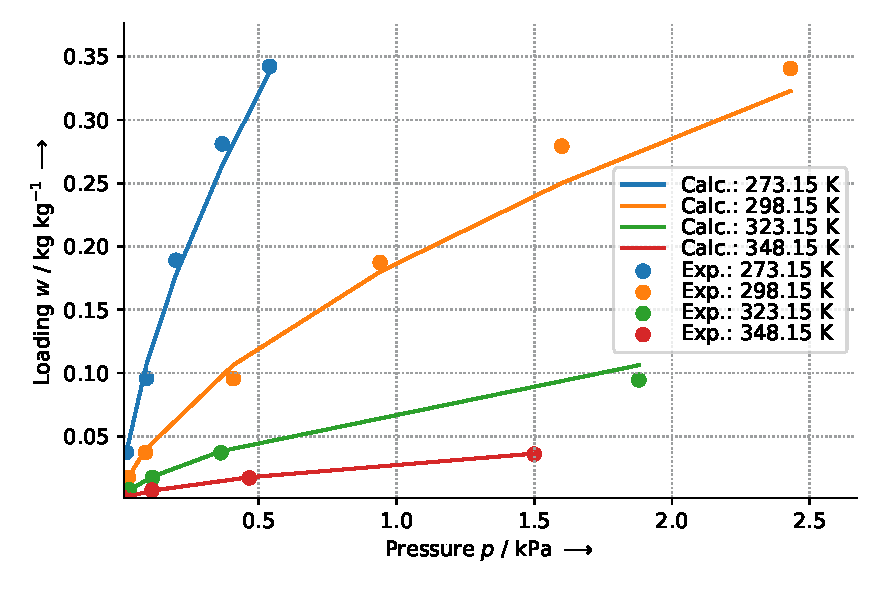
\includegraphics[height=10cm, keepaspectratio]{figs/ads/ads_Water_silica_gel_pellet__Toth_1.pdf}}
\end{figure}
%

To generate the figure, the following refrigerant functions were selected:
\begin{itemize}
\item Vapor pressure: VaporPressure\_EoS1 - ID 1
\item Saturated liquid density: SaturatedLiquidDensity\_EoS1 - ID 1
\end{itemize}

The uncertainity of the experimental data is:
\begin{itemize}
\item Data source $\,\to\,$ Data was taken from table
\item Pressure, relative, in \% $\,\to\,$ 0.067 Pa < p < 13300 Pa: 0.25% reading | 6900 Pa < p < 103000 Pa: 0.25% full scale
\item Temperature, absolute, in $\si{\kelvin}$ $\,\to\,$ 0.3
\end{itemize}

The mean absolute percentage error (MAPE) between the experimental and calculated data results in 5.36\%.
\FloatBarrier
\newpage
%%%%%%%%%%%%%%%%%%%%%%%%%%%%%%%%%%%%%%%%%%%%%%%%%%%%%%%%%%%%%%%%%%%%%%%%%%%%%%%
